\documentclass{article}

\usepackage{graphicx}
\usepackage{tikz}
\usepackage{tikzsymbols}
\usetikzlibrary{calc,patterns,shapes.geometric}
\pagestyle{empty}
\usepackage[margin=0pt]{geometry}
\geometry{papersize={14in,12in}}

\def\centerarc[#1](#2)(#3:#4:#5){\draw[#1] ($(#2)+({#5*cos(#3)},{#5*sin(#3)})$) arc (#3:#4:#5);}

\begin{document}
	\begin{figure}
		\centering
		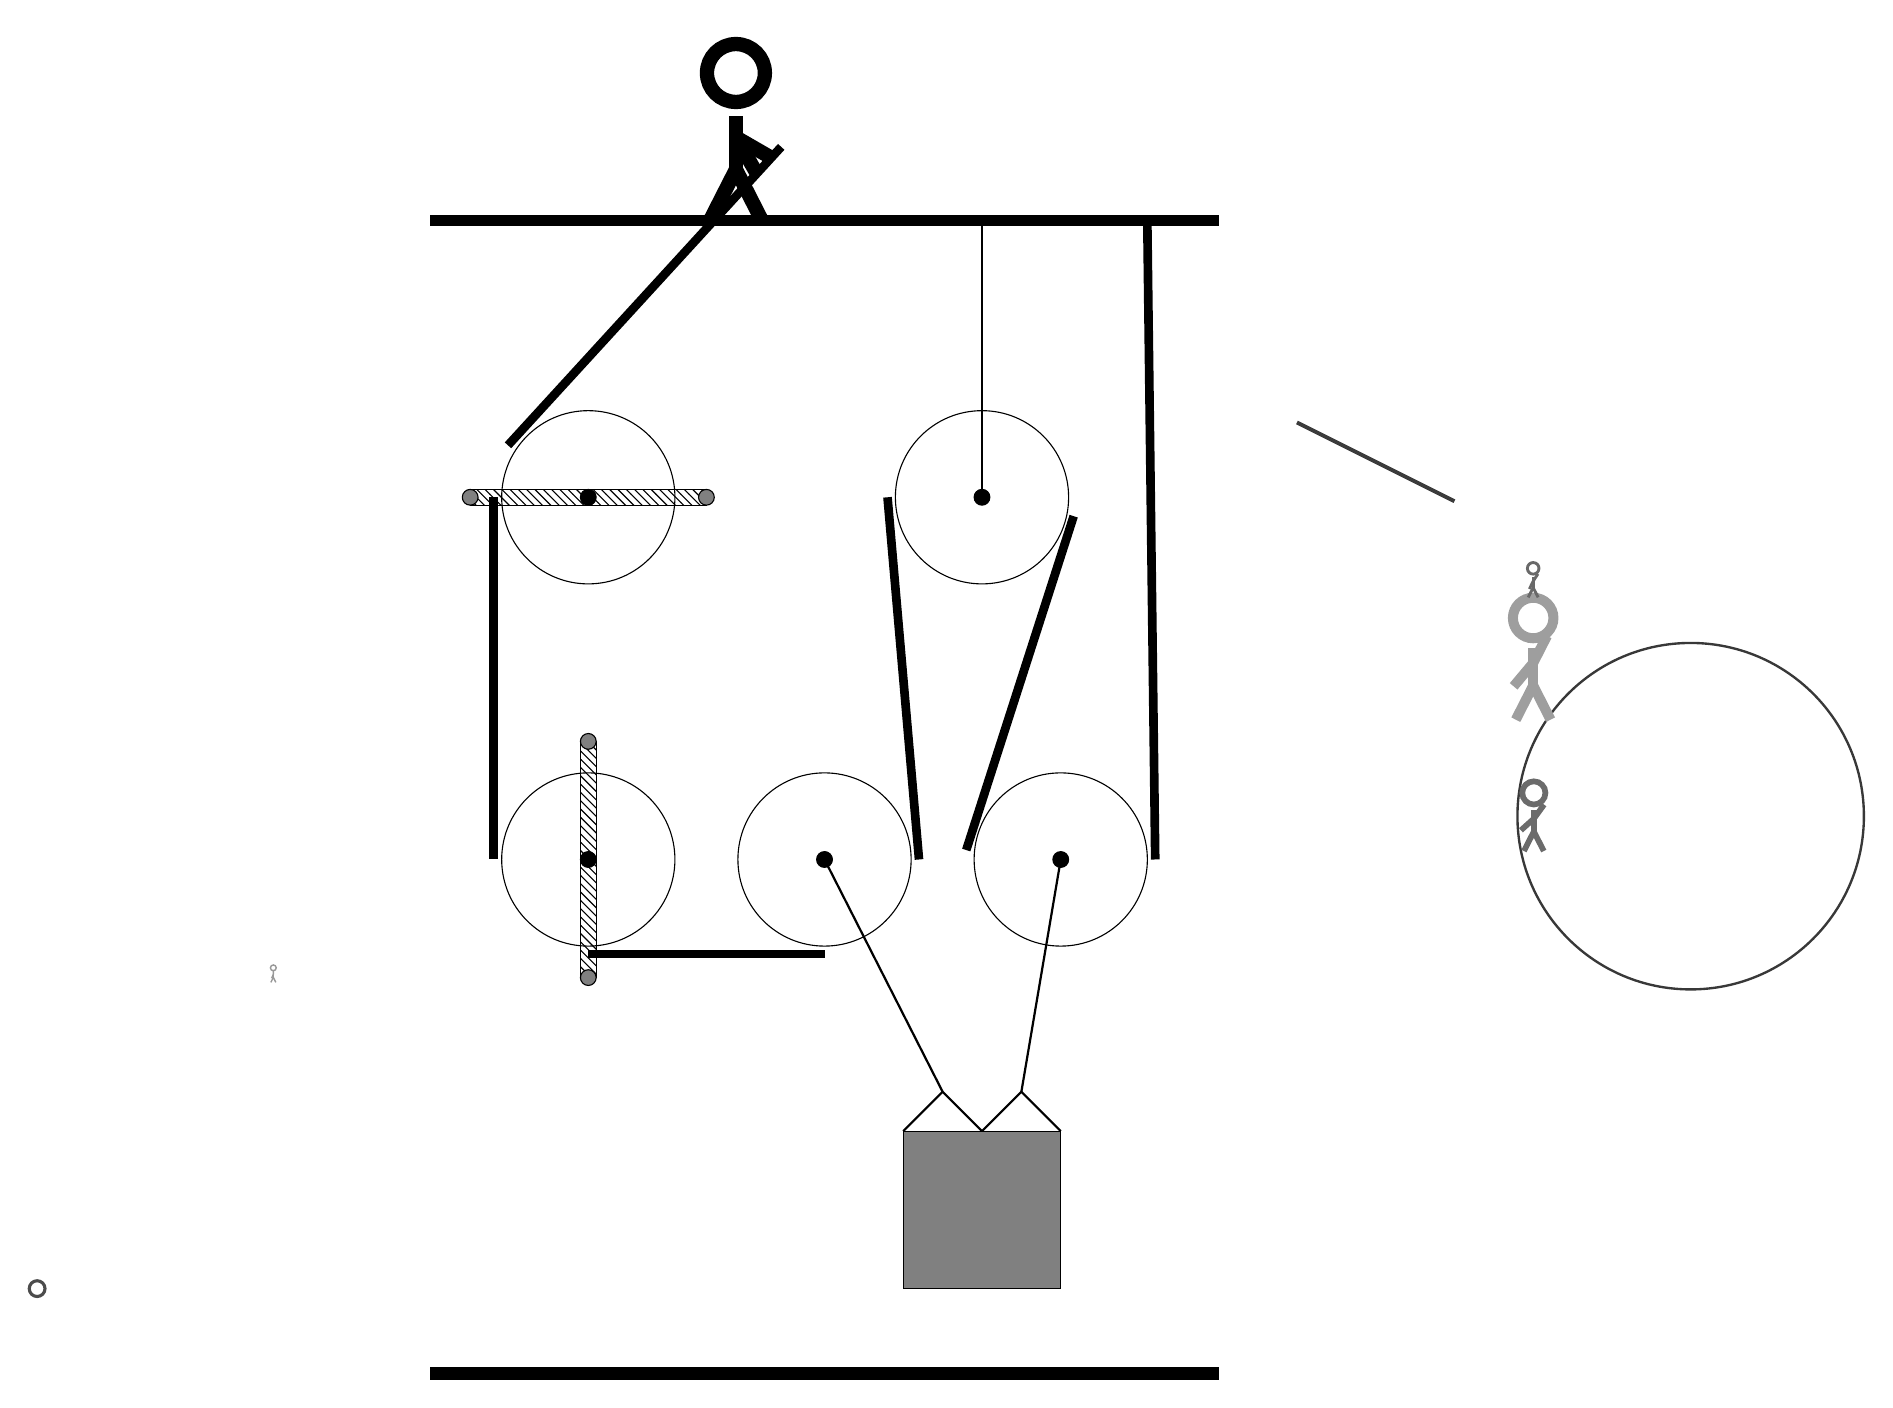
\begin{tikzpicture}
			%%%%% START %%%%%
			
			\draw[fill=black] (-4, 11.5) rectangle (6, 11.625);
			
			\draw (1, 3.45) circle (1.1);
			\draw[fill=black] (1, 3.45) circle (0.1);
			
			\draw (3, 8.05) circle (1.1);
			\draw[fill=black] (3, 8.05) circle (0.1);
			\draw[thick] (3, 8.05) -- (3, 11.5);
			
			\draw (4, 3.45) circle (1.1);
			\draw[fill=black] (4, 3.45) circle (0.1);
			
			\draw[thick] (4, 3.45) -- (3.5, 0.5);
			\draw[thick] (1, 3.45) -- (2.5, 0.5);
			\draw[thick]  (2, 0) -- (2.5, 0.5) -- (3, 0);
			\draw[thick]  (3, 0) -- (3.5, 0.5) -- (4, 0);
			\draw[fill=black!50] (2, 0) rectangle (4, -2);
			
			\draw (-2, 3.45) circle (1.1);
			\draw[fill=black] (-2, 3.45) circle (0.1);
			\draw[pattern=north west lines, pattern color=black] (-2.1, 4.95) rectangle (-1.9, 1.95);
			\draw[fill=black!50] (-2, 4.95) circle (0.1);
			\draw[fill=black!50] (-2, 1.95) circle (0.1);
			
			\draw (-2, 8.05) circle (1.1);
			\draw[fill=black] (-2, 8.05) circle (0.1);
			\draw[pattern=north west lines, pattern color=black] (-3.5, 8.15) rectangle (-0.5, 7.95);
			\draw[fill=black!50] (-3.5, 8.05) circle (0.1);
			\draw[fill=black!50] (-0.5, 8.05) circle (0.1);
			
			\draw[line width=1.1mm] (0.45, 12.5) -- (-3.02, 8.71);
			\centerarc[line width=1.1mm](-2, 8.05)(135:180:1.2000000000000002);
			\draw[line width=1.1mm] (-3.2, 8.05) -- (-3.2, 3.45);
			\centerarc[line width=1.1mm](-2, 3.45)(180:270:1.2000000000000002);
			\draw[line width=1.1mm](-2, 2.25) -- (1, 2.25);
			\centerarc[line width=1.1mm](1, 3.45)(270:360:1.2000000000000002);
			\draw[line width=1.1mm] (2.2, 3.45) -- (1.8, 8.05);
			\centerarc[line width=1.1mm](3, 8.05)(-20:180:1.2000000000000002);
			\draw[line width=1.1mm](4.164, 7.81) -- (2.8, 3.57);
			\centerarc[line width=1.1mm](4, 3.45)(160:360:1.2000000000000002);
			\draw[line width=1.1mm](5.2, 3.45) -- (5.1, 11.5);
			
			\draw [line width=0.3mm, color=black!78](12, 4) circle (2.2);
			
			\node[line width=0.6mm, color=black!38] at (10, 6) {\Strichmaxerl[7][50][63]};
			\draw[line width=0.5mm, color=black!77](7, 9) -- (9, 8);
			\node[line width=0.7mm, color=black!58] at (10, 4) {\Strichmaxerl[4][42][54]};
			
			\draw [line width=0.4mm, color=black!70](-9, -2) circle (0.1);
			\node[line width=0.3mm, color=black!59] at (10, 7) {\Strichmaxerl[2][64][57]};
			\node[line width=0.5mm, color=black!40] at (-6, 2) {\Strichmaxerl[1][67][88]};
			
			
			\node at (-0.07, 12.7) {\Strichmaxerl[10][120][-30]};
			
			\draw[fill=black] (-4, -3) rectangle (6, -3.15);
			
			%%%%% END %%%%%
		\end{tikzpicture}
	\end{figure}	
\end{document}